\chapter{Moca}

%\usepackage{graphics} is needed for \includegraphics
\begin{figure}[htp]
\begin{center}
 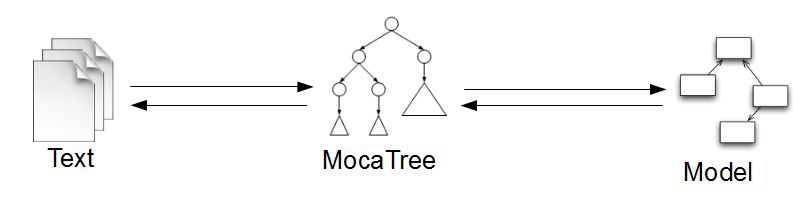
\includegraphics[width=\textwidth]{pics/moca/overview}
  \caption{Overview of model-to-text with the MOCA framework}
  \label{moca-overview}
\end{center}
\end{figure} 
 
%\usepackage{graphics} is needed for \includegraphics
\begin{figure}[htp]
\begin{center}
 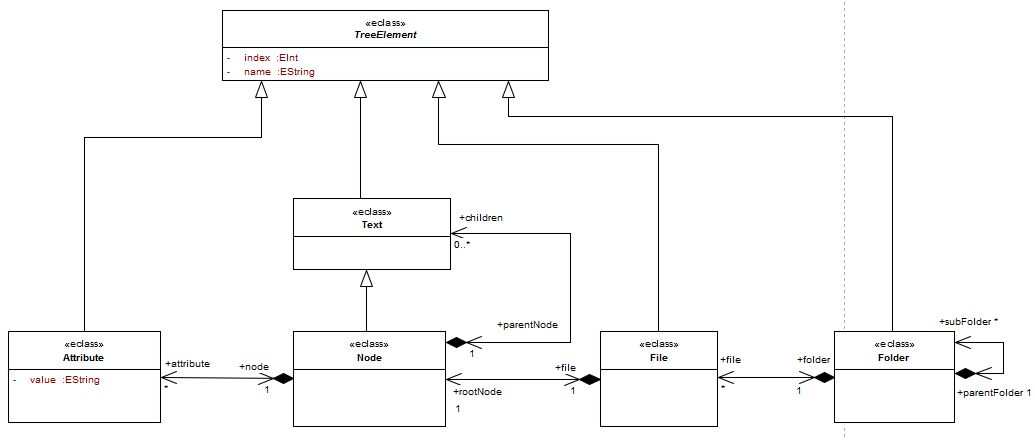
\includegraphics[width=\textwidth]{pics/moca/0Install/0-MocaTree}
  \caption{MocaTree metamodel}
  \label{moca-mocatree}
\end{center}
\end{figure}  
 
%\usepackage{graphics} is needed for \includegraphics
\begin{figure}[htp]
\begin{center}
 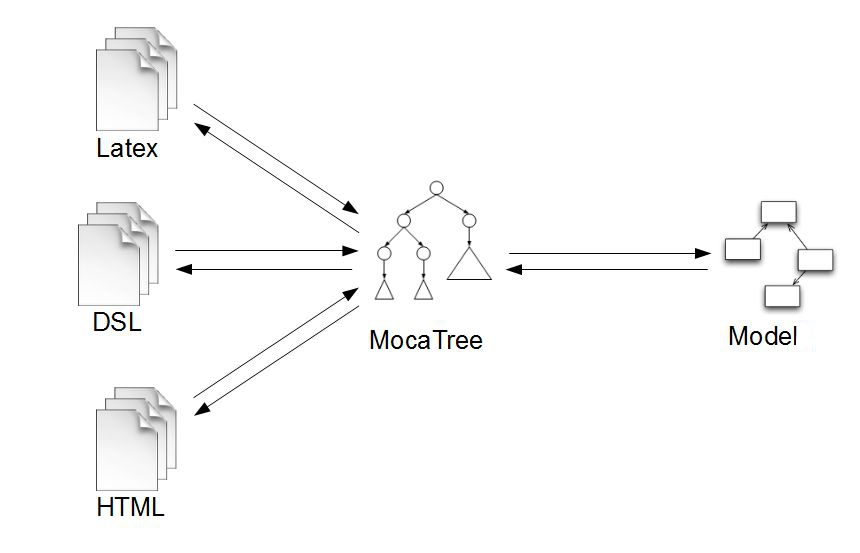
\includegraphics[width=\textwidth]{pics/moca/text-all}
  \caption{Overview of model-to-text with different text representations}
  \label{moca-text-all}
\end{center}
\end{figure}

\section{ANTLR}

%\usepackage{graphics} is needed for \includegraphics
\begin{figure}[htp]
\begin{center}
 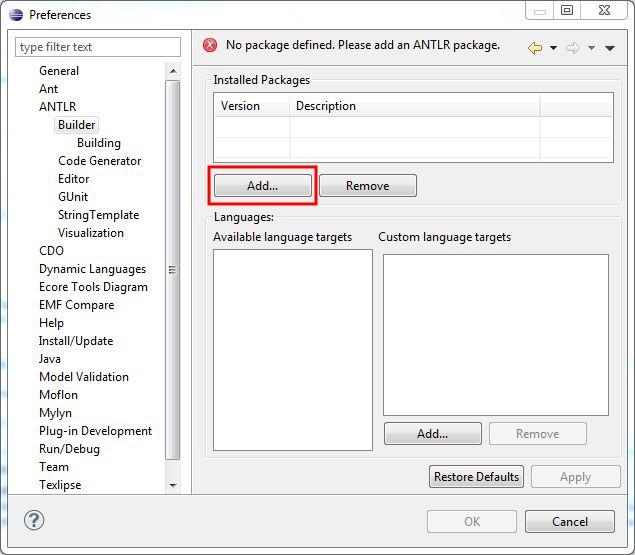
\includegraphics[width=\textwidth]{pics/moca/0Install/1-antlr-package}
  \caption{ANTLR installation: Builder preferences}
  \label{moca-1-antlr-package}
\end{center}
\end{figure}

%\usepackage{graphics} is needed for \includegraphics
\begin{figure}[htp]
\begin{center}
 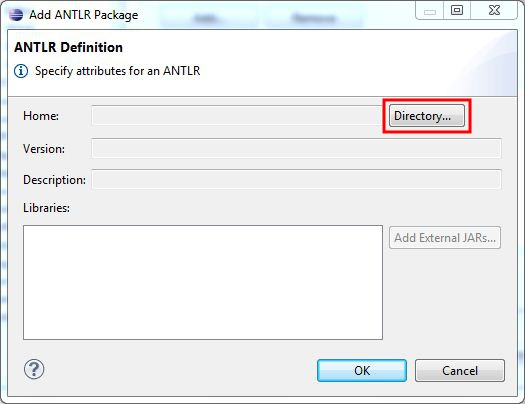
\includegraphics[width=0.7\textwidth]{pics/moca/0Install/2-choose-path-to-jar}
  \caption{ANTLR installation: dialog for choosing ANTLRworks as builder}
  \label{moca-2-choose-path-to-jar}
\end{center}
\end{figure}

Install the ANTLR eclipse plugin from
\url{http://antlrv3ide.sourceforge.net/updates}

Download ANTLRworks (\url{http://www.antlr.org/works/index.html})
\url{www.antlr.org/download/antlrworks-1.4.3.jar}

Add ANTLR Package:
- Window $>$ Preferences $>$ ANTLR $>$ Builder 
- Choose ``Add'' (see Fig. \ref{moca-1-antlr-package})
- Choose ``Directory'' and browse to the directory with the downloaded
ANTLRworks jar (see Fig. \ref{moca-2-choose-path-to-jar})

\section{Workspace for Model-to-Text Transformation}

- Start Eclipse with empty Workspace
- Switch to the moflon perspective

%\usepackage{graphics} is needed for \includegraphics
\begin{figure}[!htbp]
\begin{center}
 
\includegraphics[width=0.3\textwidth]{pics/moca/1DictionaryMetaModel/1-NewMetamodelWizard}
  \caption{Opening the ``New Metamodel'' wizard}
  \label{moca-1-NewMetamodelWizard}
\end{center}
\end{figure}

- Open the ``New Metamodel'' wizard 

%\usepackage{graphics} is needed for \includegraphics
\begin{figure}[!htbp]
\begin{center}
 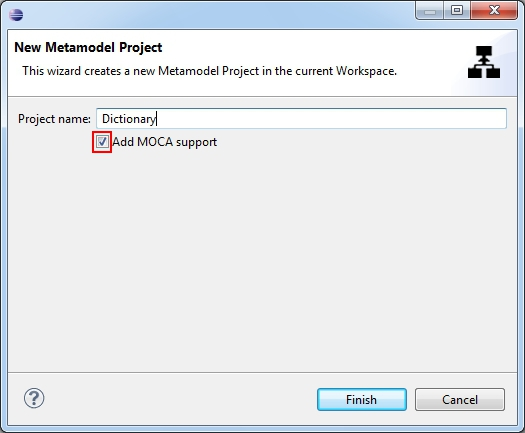
\includegraphics[width=0.7\textwidth]{pics/moca/1DictionaryMetaModel/2-AddMocaSupport-ProjectName}
  \caption{Add Metamodel project with MOCA support}
  \label{moca-2-AddMocaSupport-ProjectName}
\end{center}
\end{figure}

- Set project name to ``Dictionary''
- Select "Add Moca Support" 


%\usepackage{graphics} is needed for \includegraphics
\begin{figure}[!htbp]
\begin{center}
 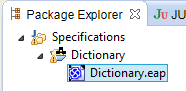
\includegraphics[width=0.3\textwidth]{pics/moca/1DictionaryMetaModel/3-WizardResult}
  \caption{Workspace after wizard finishes}
  \label{moca-3-WizardResult}
\end{center}
\end{figure}

- Project and eap file are created (see Fig. \ref{moca-3-WizardResult})

%\usepackage{graphics} is needed for \includegraphics
\begin{figure}[!htbp]
\begin{center}
 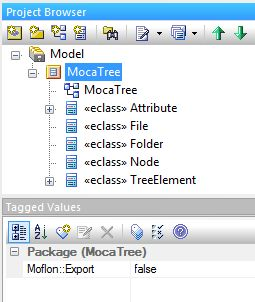
\includegraphics[width=0.5\textwidth]{pics/moca/1DictionaryMetaModel/4-eapContainsMocatreeWithExportFalse}
  \caption{The EA project contains a package ``MocaTree'' with property
  $Moflon::Export = false$}
  \label{moca-4-eapContainsMocatreeWithExportFalse}
\end{center}
\end{figure}

- open Dictionary.eap
- eap file contains MocaTree package with $export = false$ (Fig.
\ref{moca-4-eapContainsMocatreeWithExportFalse})

\begin{figure}[!htbp]
\begin{center}
 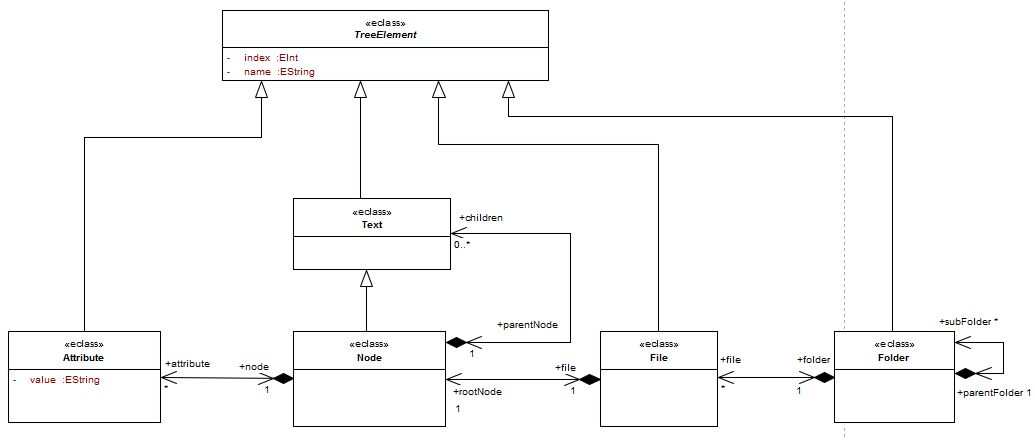
\includegraphics[width=\textwidth]{pics/moca/0Install/0-MocaTree}
  \caption{Mocatree metamodel}
  \label{moca-tree}
\end{center}
\end{figure}
 

%\usepackage{graphics} is needed for \includegraphics
\begin{figure}[!htbp]
\begin{center}
 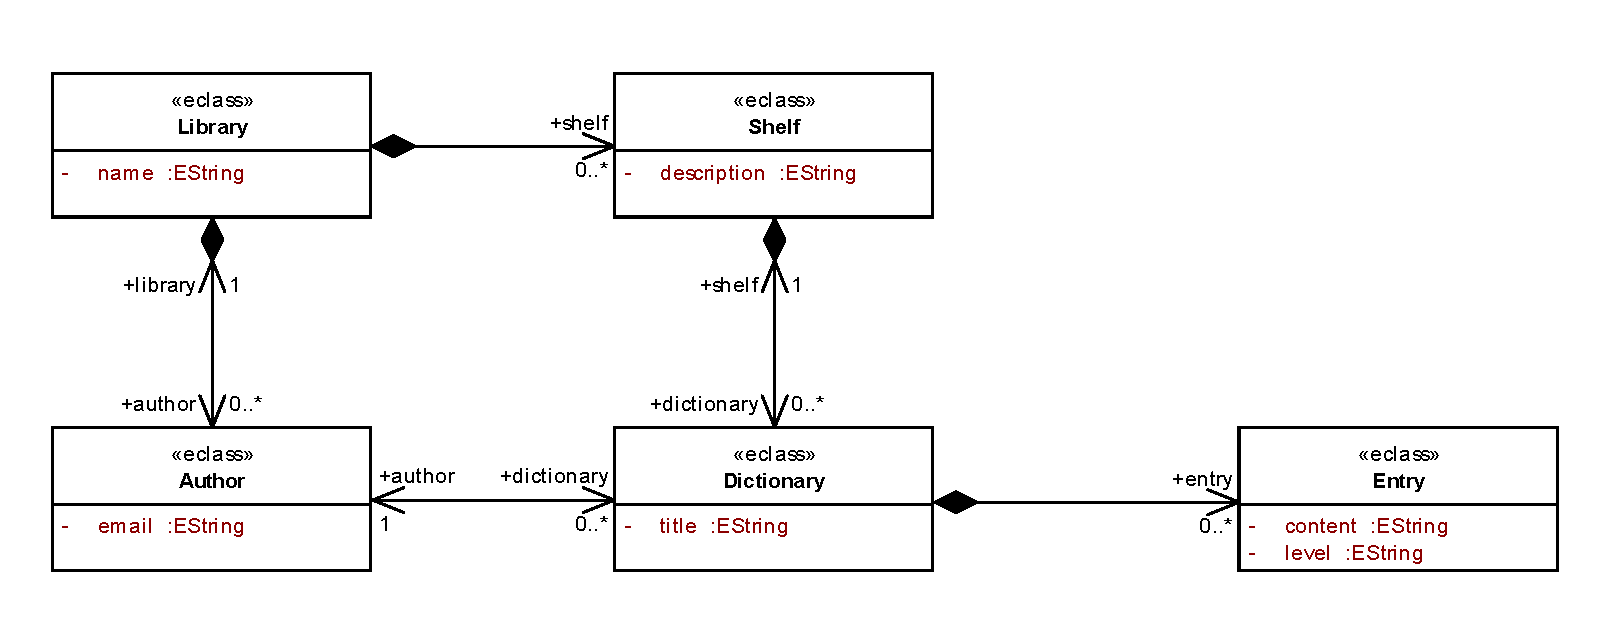
\includegraphics[width=\textwidth]{pics/moca/1DictionaryMetaModel/DictionaryLanguage}
  \caption{Dictionary metamodel}
  \label{moca-5-DictionaryMM}
\end{center}
\end{figure}

- Add dictionary Metamodel like in (Fig. \ref{moca-5-DictionaryMM})
- Add package ``DictionaryCodeAdapter''

%\usepackage{graphics} is needed for \includegraphics
\begin{figure}[!htbp]
\begin{center}
 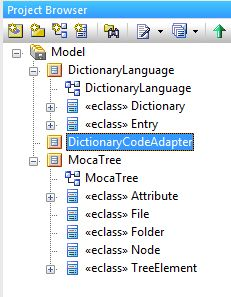
\includegraphics[width=0.5\textwidth]{pics/moca/1DictionaryMetaModel/5-DictionaryMM-ProjectBrowser}
  \caption{EA project view before exporting}
  \label{moca-5-DictionaryMM-ProjectBrowser}
\end{center}
\end{figure}

- EA projects just before export (Fig. \ref{moca-5-DictionaryMM-ProjectBrowser}) 

%\usepackage{graphics} is needed for \includegraphics
\begin{figure}[!htbp]
\begin{center}
 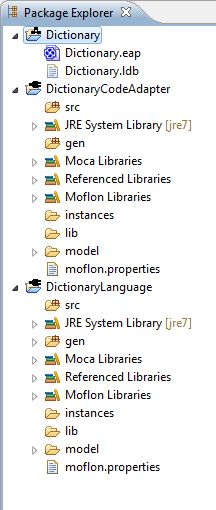
\includegraphics[width=0.3\textwidth]{pics/moca/1DictionaryMetaModel/6-ExportToEclipse}
  \caption{Workspace after export to eclipse}
  \label{moca-6-ExportToEclipse}
\end{center}
\end{figure}

- Export to eclipse  (Fig. \ref{moca-6-ExportToEclipse})


%\section{Text-to-Tree Transformation}

As we shall see in a moment, libraries and shelves correspond to a folder structure while the contents for a single dictionary are specified in a file.
Figure \ref{fig:moca-4-Tokens} depicts a small sample of the textual syntax used to specify a dictionary.
On the way to an instance model of our dictionary metamodel, the very first step is to create nice \emph{chunks} of characters.
This is called \emph{lexing} and is a step that simplifies the actual comprehension of the complete text.
Interestingly human beings actually comprehend text in a similar manner, one recognizes whole words without ``seeing'' every individual character.
This is the reason why you can siltl raed tihs sneentce alsomt eforftlsesly.   
A lexer recognizes these chunks or \emph{tokens} and passes them on as a token stream to the \emph{parser} that does the actual work of recognizing complex hierarchical and recursive structures.
   
To recognize the tokens as indicated in Fig.~\ref{fig:moca-4-Tokens}, \texttt{ANTLR} can automatically generate a lexer in Java from a compact specification as depicted in Fig.~\ref{fig:moca-6-lexer}.
This is actually a DSL for lexing and is explained in detail in \cite{ANTLR}.
If you do not know what EBNF is and have problems understanding the lexer grammar then make sure you at least go through the documentation on \url{www.antlr.org} or read relevant chapters in \cite{ANTLR}.

 
%\usepackage{graphics} is needed for \includegraphics
\begin{figure}[!htbp]
\begin{center}
 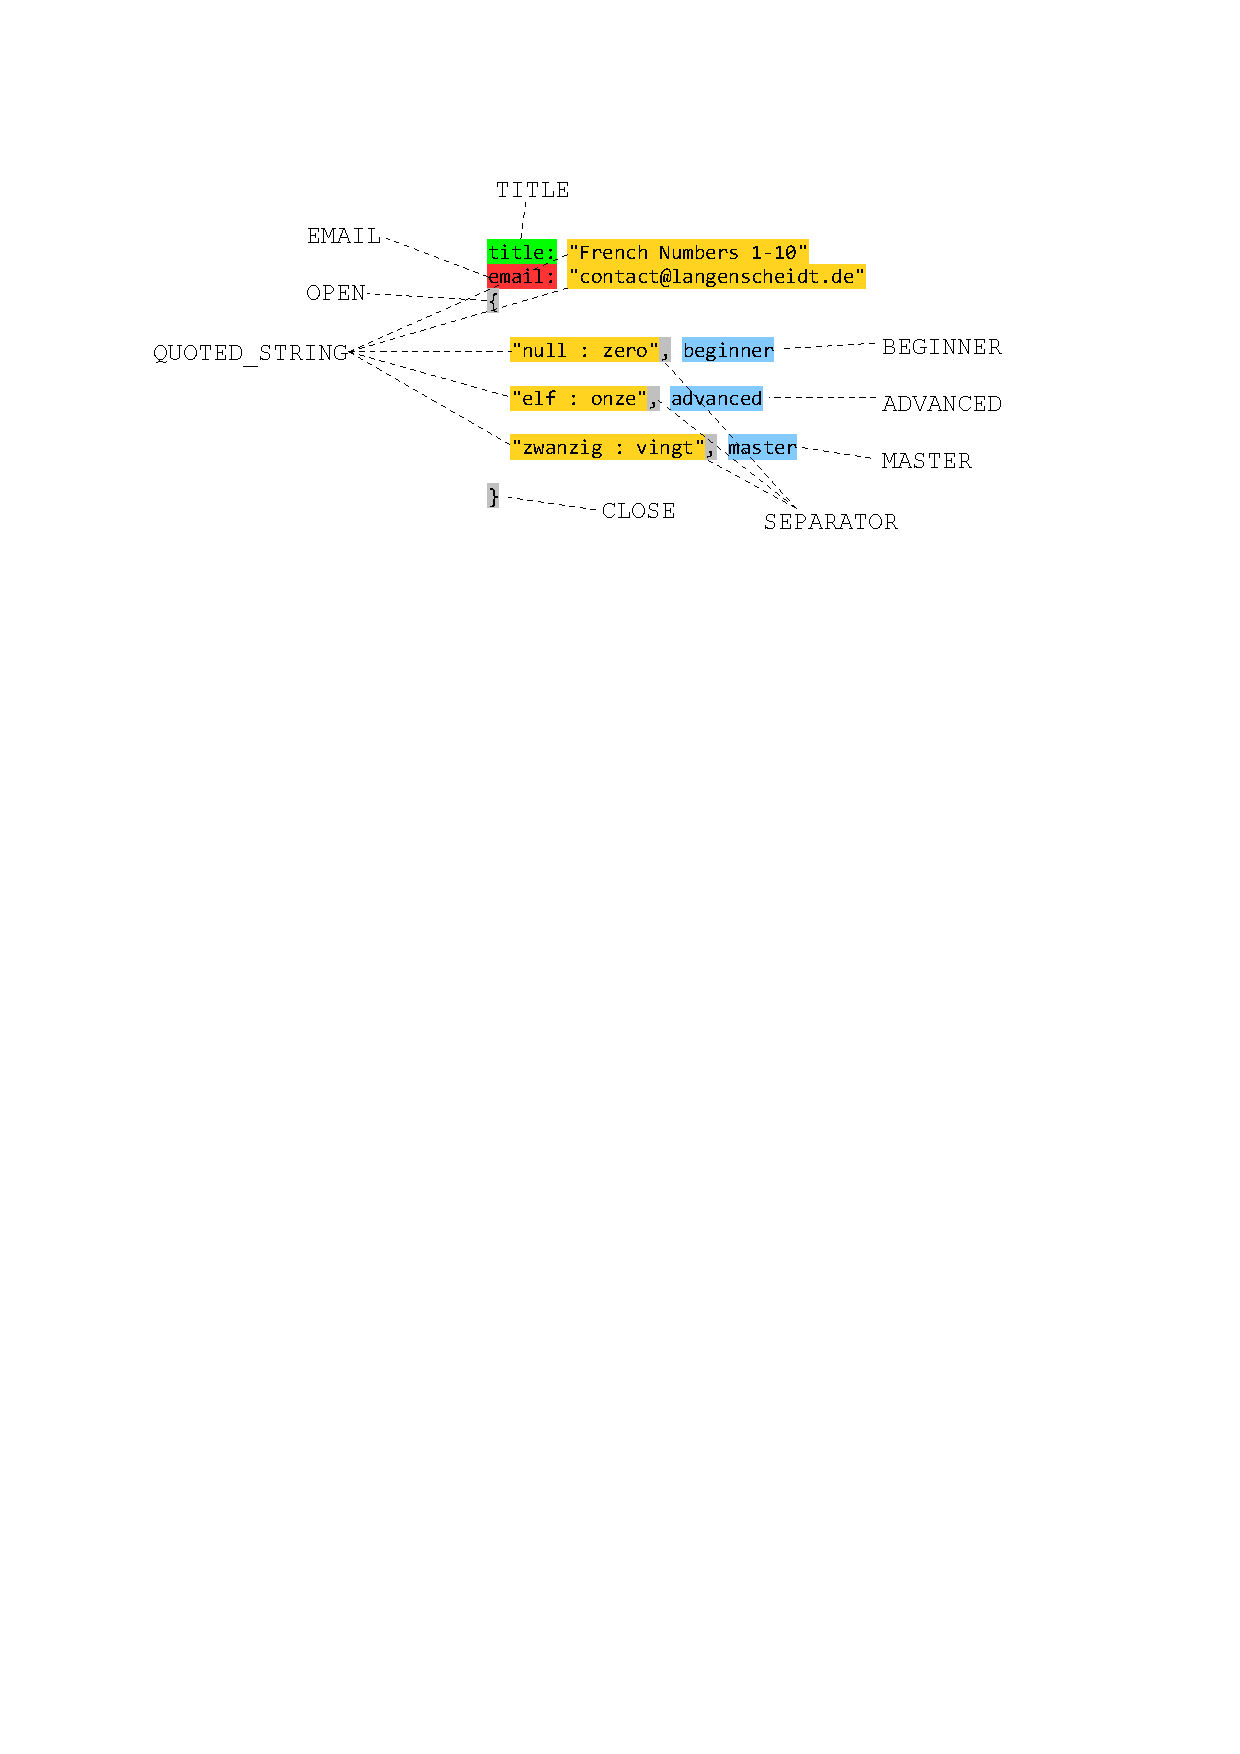
\includegraphics[width=0.8\textwidth]{pics/moca/2TextToMocaTree/4-tokens}
  \caption{Identified tokens in a dictionary file.}
  \label{fig:moca-4-Tokens}
\end{center}
\end{figure}

\begin{enumerate}
\item[$\blacktriangleright$] Edit \texttt{DictionaryLexer.g} so it closely resembles Fig.~\ref{fig:moca-6-lexer}.
Be careful to avoid any typos and mistakes.  Save and make sure it compiles.  
\end{enumerate}

%\usepackage{graphics} is needed for \includegraphics
\begin{figure}[!htbp]
\begin{center}
 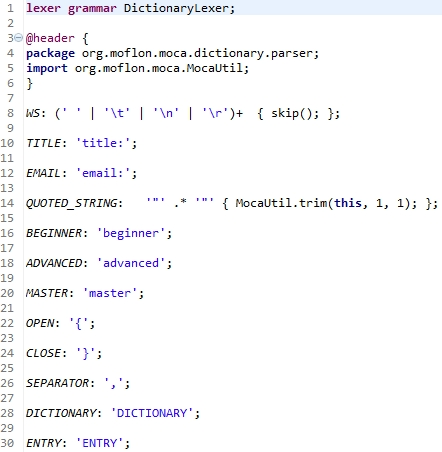
\includegraphics[width=0.75\textwidth]{pics/moca/2TextToMocaTree/6-lexer}
  \caption{Lexer grammar}
  \label{fig:moca-6-lexer}
\end{center}
\end{figure}

The next step is to form the stream of tokens from the lexer into a \emph{tree}.
In this context, a tree is an acyclic, hierarchical, recursive structure as depicted in Fig.~\ref{fig:moca-5-Tree}.
Depending on what the tree is to be used for, it can be structured very differently with \emph{imaginary} nodes like \texttt{DICTIONARY} or \texttt{ENTRY} that were not present in the textual syntax and are used to give additional structure to the tree. 

%\usepackage{graphics} is needed for \includegraphics
\begin{figure}[htp]
\begin{center}
 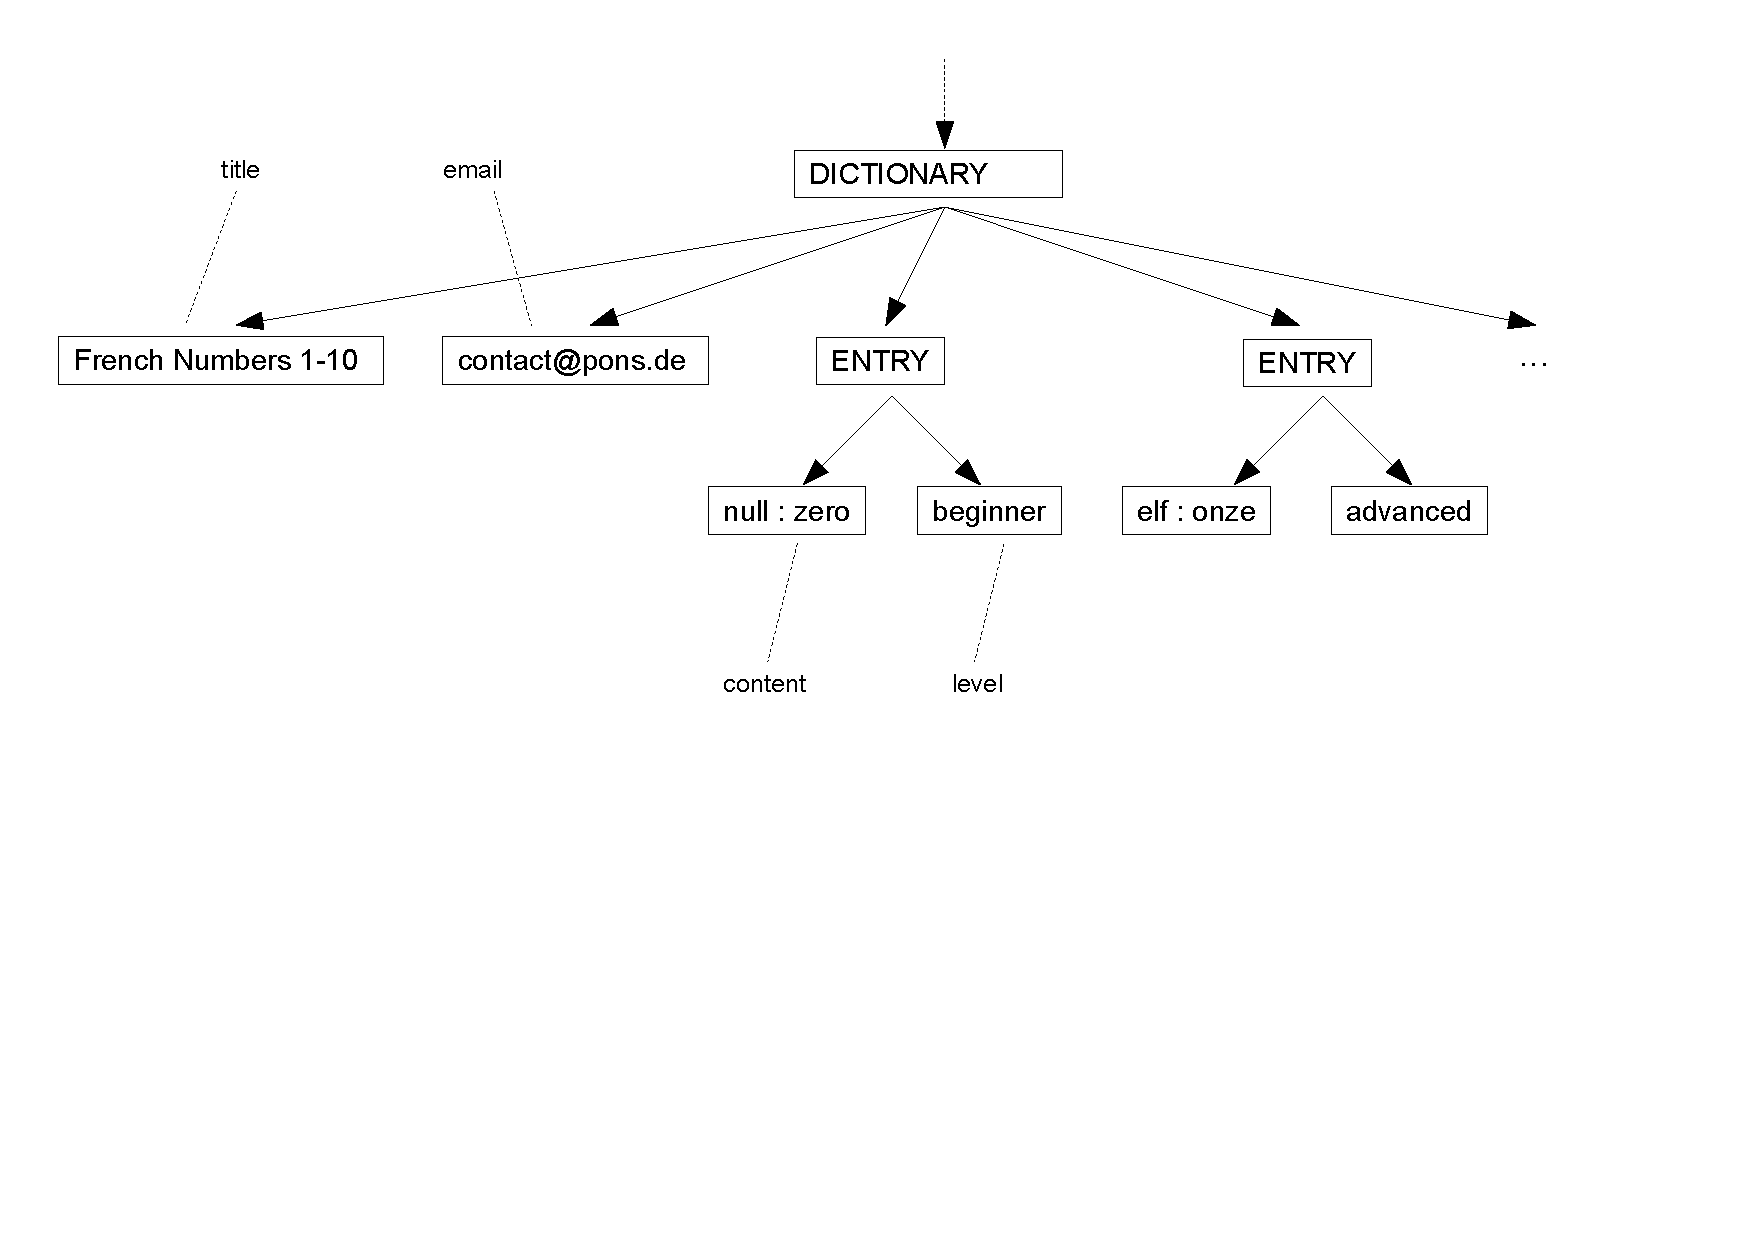
\includegraphics[width=\textwidth]{pics/moca/2TextToMocaTree/5-tree}
  \caption{MocaTree structure}
  \label{fig:moca-5-Tree}
\end{center}
\end{figure}

\begin{enumerate}
\item[$\blacktriangleright$] Edit \texttt{DictionaryParser.g} so it closely resembles Fig.~\ref{fig:moca-7-parser}.
As with the lexer, avoid typos and mistakes and make sure it compiles.
\end{enumerate}

%\usepackage{graphics} is needed for \includegraphics
\begin{figure}[!htbp]
\begin{center}
 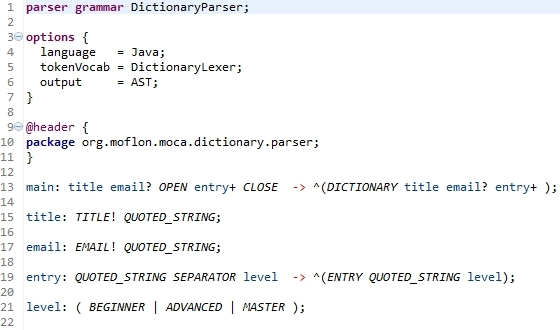
\includegraphics[width=0.9\textwidth]{pics/moca/2TextToMocaTree/7-parser}
  \caption{Parser grammar}
  \label{fig:moca-7-parser}
\end{center}
\end{figure}
The parser grammar is quite similar to the lexer grammar, but there are \emph{parser actions} after \texttt{->} to build up the tree.
Using this simple tree language, one can (1) abstract from tokens like \texttt{\{} or \texttt{\}}, which are just \emph{syntactical noise} and (2) enrich the tree with imaginary nodes like \texttt{ENTRY}, which add explicit structure to the tree.
Please refer to \cite{ANTLR} and online resources for a detailed explanation of the syntax and semantics of the parser grammar supported by \texttt{ANTLR}. 
 
%\usepackage{graphics} is needed for \includegraphics
\begin{figure}[htp]
\begin{center}
 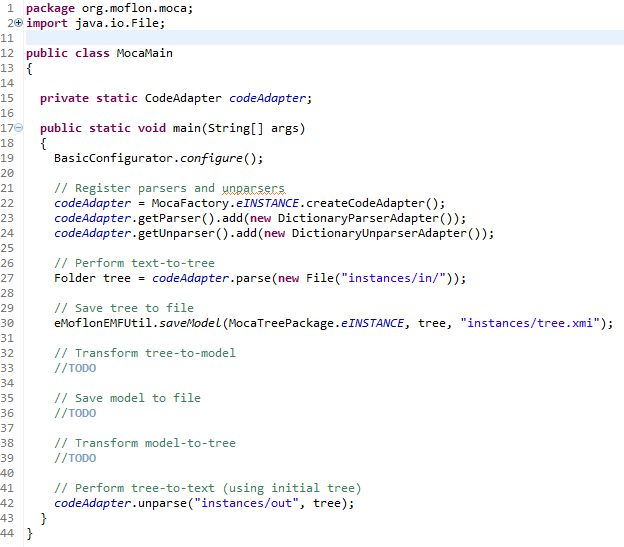
\includegraphics[width=\textwidth]{pics/moca/2TextToMocaTree/8-MocaMain}
  \caption{Generated main method}
  \label{fig:moca-8-MocaMain}
\end{center}
\end{figure}

Before we take our lexer and parser for a spin, open \texttt{MocaMain.java} and inspect it.
If everything went right it should bear a striking resemblance to Fig.~\ref{fig:moca-8-MocaMain}.
For the moment we do not need to adjust anything, just note how the parser is added to the Moca framework (line 23) via an adapter (\texttt{Dictionary\-Parser\-Adapter}).
Go ahead and look at what the adapter exactly does.
All the code can be adjusted and used to, for example, define which files the parser is to be used for (per default the adapter registers for \texttt{*.dictionary} files).
The main job of the adapter is to hide \texttt{ANTLR} specifics so the framework remains (parser) technology agnostic.
If you decide to use a different parser generator or write the parser by hand you would need to implement a corresponding adapter from scratch.

On line 27, the input for the framework is set, meaning that all folders in \texttt{./instances/in} are parsed.
In a nutshell, each folder is taken as a root of a tree and the folder and file structure is reflected as a hierarchy of (children)nodes in the tree.
For each file, the framework searches for a registered parser that is responsible for the particular file, passes the content on to the parser and plugs in the tree from the parser as a single subtree of the corresponding file node in the overall tree.  Take a look at Fig.~\ref{fig:moca-overview} again and review the parts we have covered.

The final step is now to prepare some input for the framework:
\begin{enumerate}
  \item[$\blacktriangleright$] Create the directory structure depicted in Fig.~\ref{fig:moca-inputdata} in \texttt{Dictionary\-Code\-Adapter} and enter the contents from Table~\ref{moca-inputdata} for each of the four \texttt{dictionary} files\footnote{You can just copy\&paste right from the PDF file}.
  %\usepackage{graphics} is needed for \includegraphics
\begin{figure}[htp]
\begin{center}
  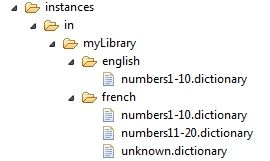
\includegraphics[width=0.45\textwidth]{pics/moca/2TextToMocaTree/inputData}
  \caption{Input directory structure.}
  \label{fig:moca-inputdata}
\end{center}
\end{figure}
\vspace{-0.5cm}
\item[$\blacktriangleright$] After creating all the dictionaries, run \texttt{MocaMain.java} as a normal Java application. If everything works out right, a \texttt{tree.xmi} and an \texttt{out} folder should be created in \texttt{instances}.  Inspect their contents and compare to Fig.~\ref{fig:moca-9-ParseResult1}. The unparsed files are obviously empty as we haven't implemented an \emph{unparser} yet.
%\usepackage{graphics} is needed for \includegraphics
\begin{figure}[htp]
\begin{center}
 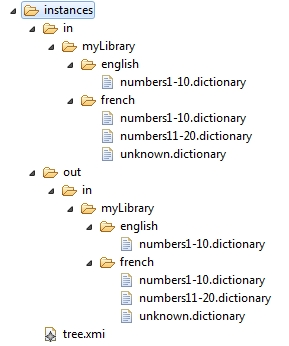
\includegraphics[width=0.45\textwidth]{pics/moca/2TextToMocaTree/9-ParseResult1}
  \caption{Directory \texttt{instances} after parsing}
  \label{fig:moca-9-ParseResult1}
\end{center}
\end{figure} 
\end{enumerate}
\clearpage

\begin{table}
\begin{tabular}{p{6cm} p{6cm} }
\footnotesize
\textbf{english/numbers1-10.dictionary:}
\begin{verbatim}
title: "English Numbers 1-10"
email: "contact@langenscheidt.de"	
{
  "null : zero", beginner
  "eins : one", beginner
  "zwei : two", beginner
  "drei : three", beginner
  "vier : four", beginner
  "fuenf : five", beginner
  "sechs : six", beginner
  "sieben : seven", beginner
  "acht : eight", beginner
  "neun : nine", beginner
  "zehn : ten", beginner 
}
\end{verbatim} 

\textbf{french/numbers1-10.dictionary:}
\begin{verbatim}   
title: "French Numbers 1-10"
email: "contact@pons.de"	
{
  "null : zero", beginner
  "eins : un/une", beginner
  "zwei : deux", beginner
  "drei : trois", beginner
  "vier : quatre", beginner
  "fuenf : cinq", beginner
  "sechs : six", beginner
  "sieben : sept", beginner
  "acht : huit", beginner
  "neun : neuf", beginner
  "zehn : dix", beginner 
}
\end{verbatim}
&

\footnotesize
\textbf{french/numbers11-20.dictionary:}
\begin{verbatim}
title: "French Numbers 11-20"
email: "contact@pons.de"	
{
  "elf : onze", advanced
  "zwoelf : douze", advanced
  "dreizehn : treize", advanced
  "vierzehn : quatorze", advanced
  "fuenfzehn : quinze", advanced
  "sechzehn : seize", master
  "siebzehn : dix-sept", master
  "achtzehn : dix-huit", master
  "neunzehn : dix-neuf", master
  "zwanzig : vingt", master
}

\end{verbatim}
\textbf{french/unknown.dictionary:}
\begin{verbatim}
title: "unknown"
{
  "unbekannt", beginner
}
\end{verbatim}
  \\
\end{tabular}   
\caption{Input files containing dictionaries.}
\label{moca-inputdata}

\end{table}   

\clearpage

\begin{enumerate}
  \item[$\blacktriangleright$] Double-click \texttt{tree.xmi}\footnote{Depending on the plugins you have installed, you might have to explicitly choose \texttt{Open With/Sample Reflective Ecore Model Editor}.} and compare the contents to Fig.~\ref{fig:moca-10-ParseResult2}. At this point, you can reflect on the structure of the tree and note the directory structure, file nodes and the subtrees from the parser.
%\usepackage{graphics} is needed for \includegraphics
\begin{figure}[htp]
\begin{center}
 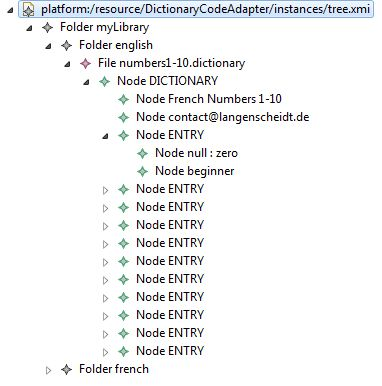
\includegraphics[width=0.7\textwidth]{pics/moca/2TextToMocaTree/10-ParseResult2}
  \caption{MocaTree created by Parser}
  \label{fig:moca-10-ParseResult2}
\end{center}
\end{figure}
\end{enumerate}

If everything worked out then well done!  We now have a nice tree that we can work on with SDMs and transform in a few simple steps to an actual instance of our Dictionary metamodel.

%\section{Tree-to-Model Transformation with SDMs}

The next step in the text-to-model transformation is a set of SDMs that transform our tree to an instance of our dictionary metamodel.
Take a look at the overview (Fig.~\ref{fig:moca-overview}) again and try to identify which arrow depicts exactly this \emph{tree-to-model} transformation.
Just a short comment;  all SDMs in this section depict story patterns directly in their story nodes.
Please do not take this as a \emph{best practice}, in fact we actually recommend always extracting story patterns.
It's just easier for the tutorial to fit each SDM on a single page!

\begin{enumerate}
  \item[$\blacktriangleright$]  In the code adapter project \texttt{DictionaryCodeAdapter}, create a \texttt{Trans\-for\-mer} class with the methods and reference to the \texttt{Library} class as depicted in Fig.~\ref{fig:moca-DictionaryCodeAdapter}.
%\usepackage{graphics} is needed for \includegraphics
\begin{figure}[!htbp]
\begin{center}
 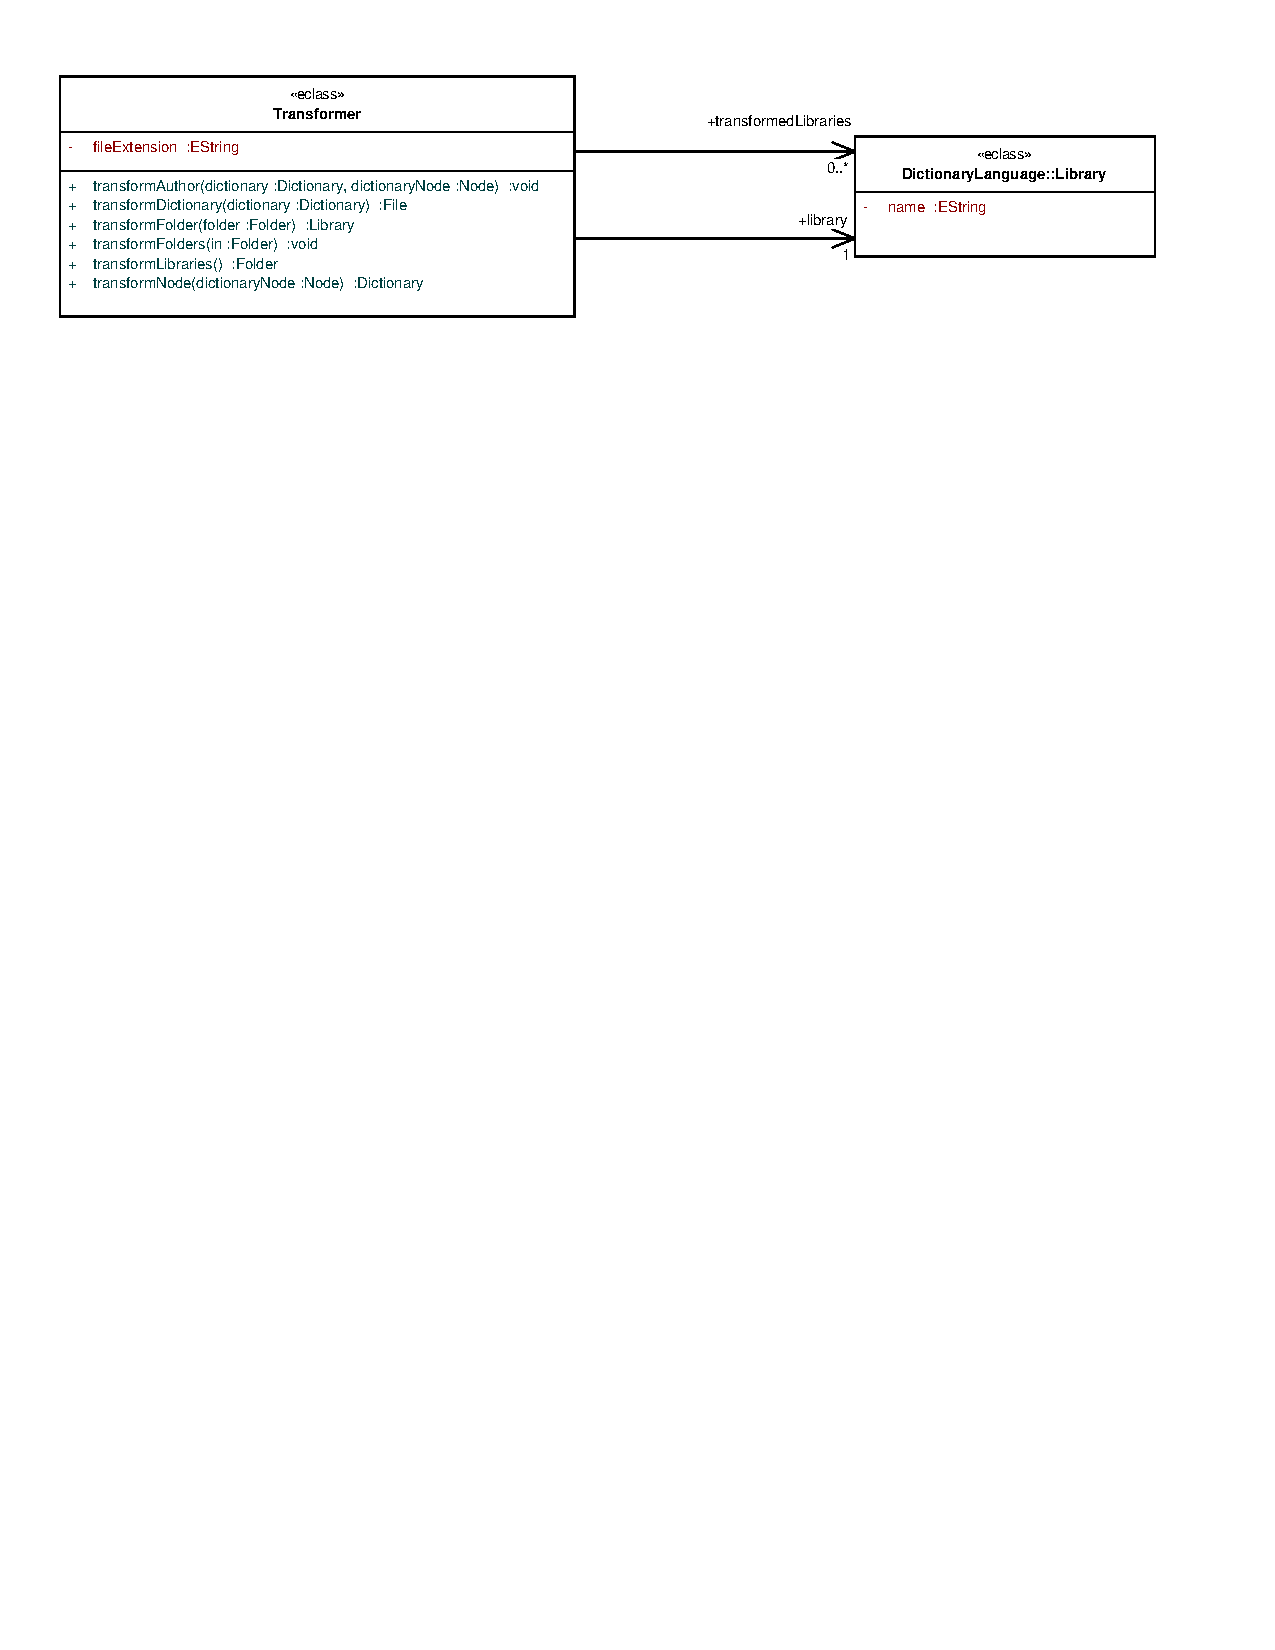
\includegraphics[width=0.9\textwidth]{pics/moca/3MocaTreeToModel/DictionaryCodeAdapter}
  \caption{Transformer class with methods for SDMs}
  \label{fig:moca-DictionaryCodeAdapter}
\end{center}
\end{figure}
\item[$\blacktriangleright$]  The first SDM \texttt{transformFolder:~Folder~$\rightarrow$~Library} is depicted in Fig.~\ref{fig:moca-transformFolder} and creates a corresponding library with shelves for the given folder, delegating the creation of dictionaries to \texttt{transformNode}.
The SDM uses features that we have treated in previous chapters.
Note that the exogenous transformation is specified by simply drag \& dropping in elements from \emph{different} metamodels as required!
All dependencies are automatically added when exporting to Eclipse -- now isn't that as simple as ABC?
%\usepackage{graphics} is needed for \includegraphics
\begin{figure}[!htbp]
\begin{center}
 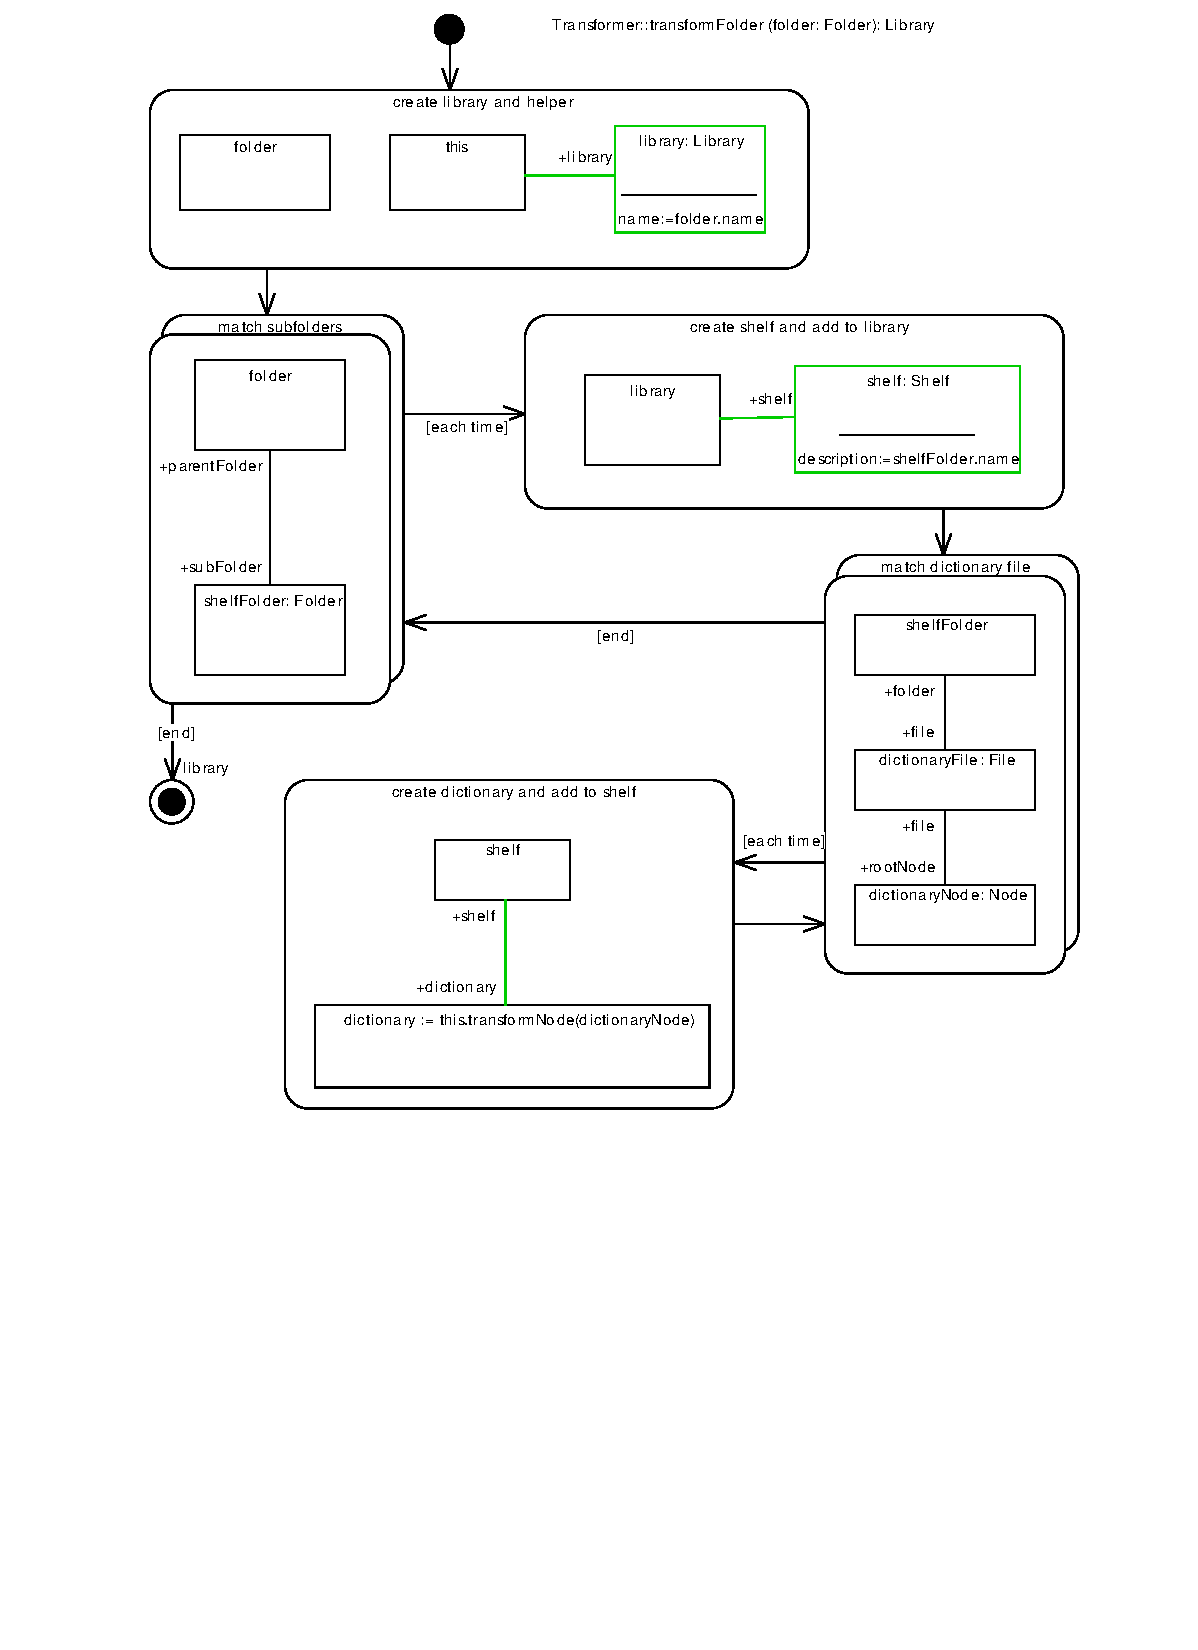
\includegraphics[width=\textwidth]{pics/moca/3MocaTreeToModel/transformFolderPrintPdf}
  \caption{Transforming the outermost folder into a dictionary}
  \label{fig:moca-transformFolder}
\end{center}
\end{figure}
\item[$\blacktriangleright$] The next SDM, \texttt{transformNode:~Node~$\rightarrow$~Dic\-tion\-ary} (Fig.~\ref{fig:moca-transformNode}) takes a node, representing a dictionary, and builds up a dictionary object adding entries appropriately.
It further delegates creation of authors to \texttt{transformAuthors}.
Note how \emph{indices} are used in the story node \texttt{match entry node} to decide, according to convention (how we built the tree), which node in the tree is to be interpreted as content and which as the level of the entry.
%\usepackage{graphics} is needed for \includegraphics
\begin{figure}[!htbp]
\begin{center}
 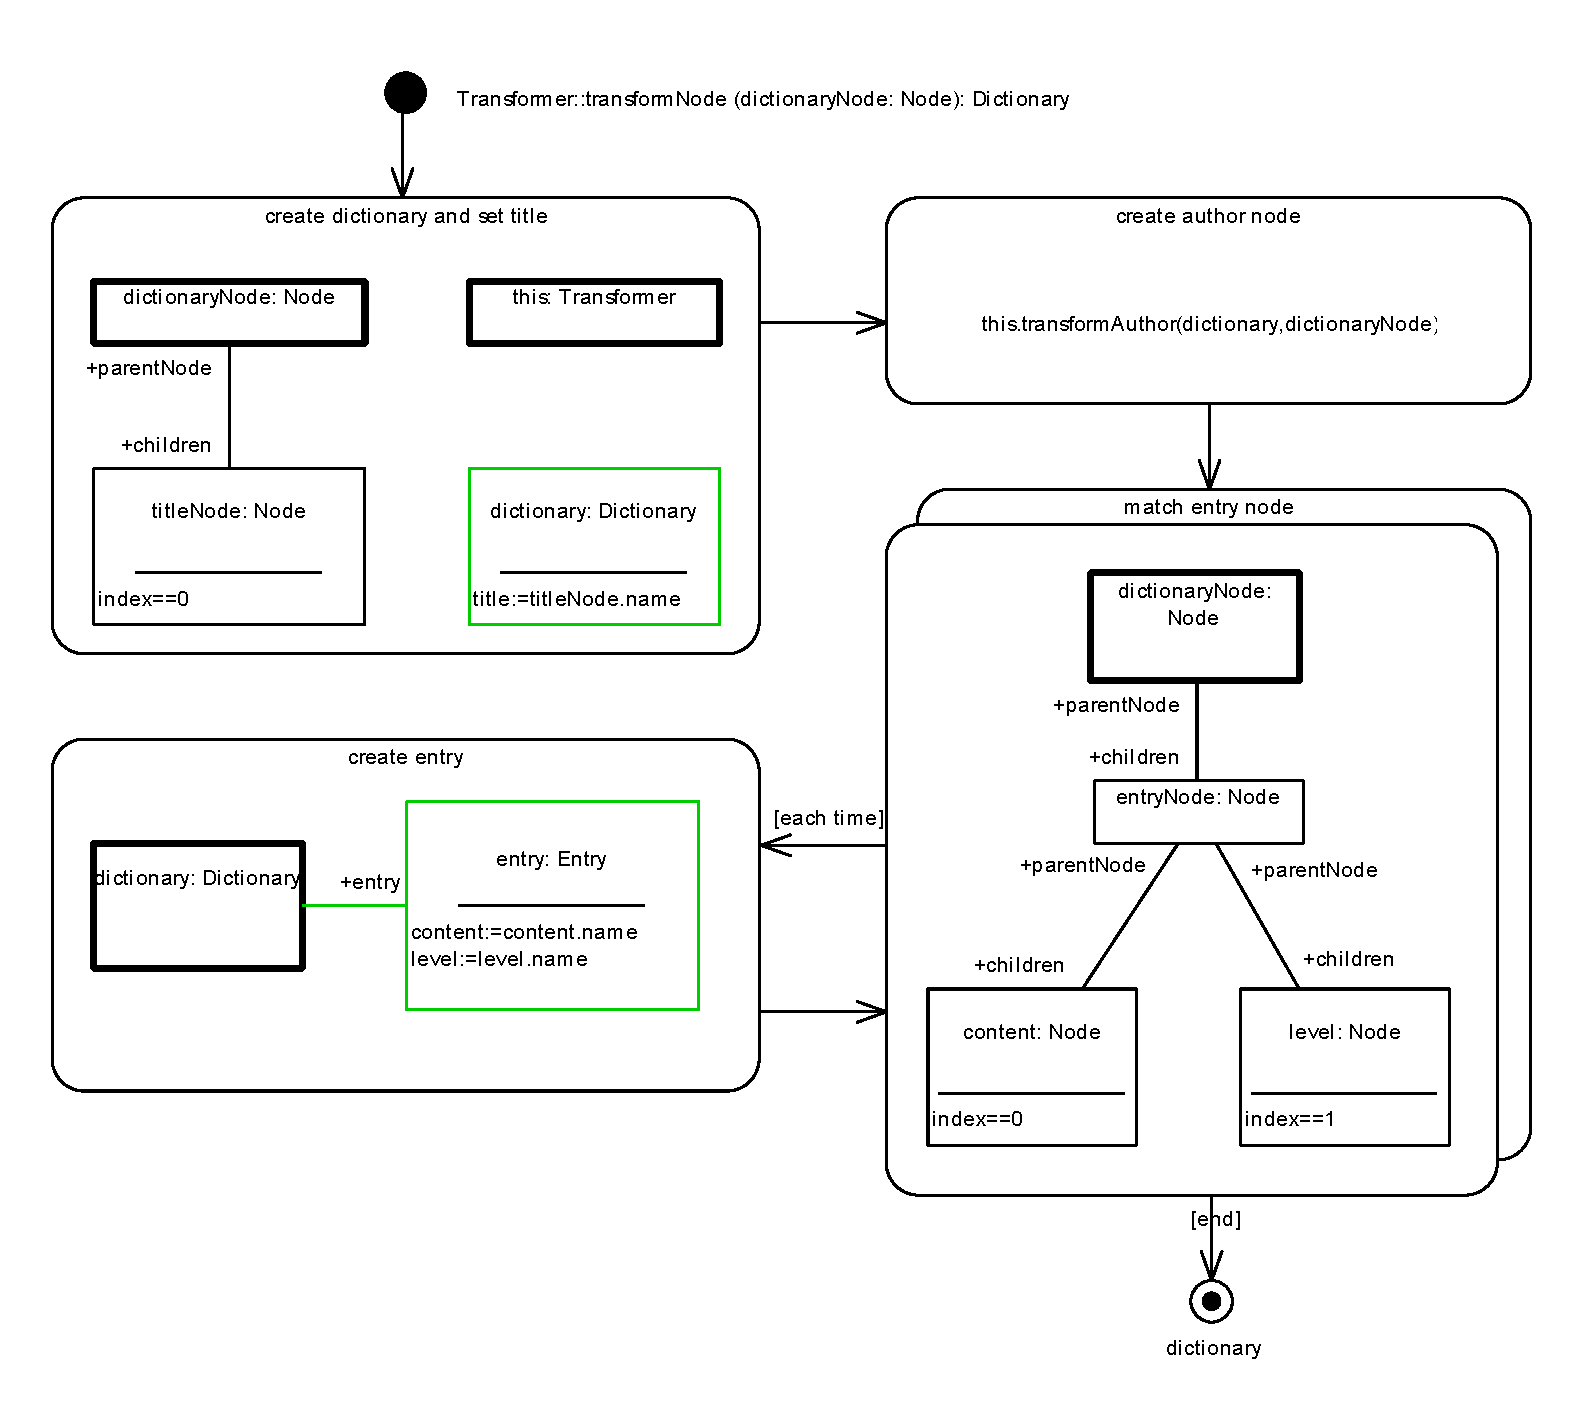
\includegraphics[width=\textwidth]{pics/moca/3MocaTreeToModel/transformNodePrintPdf}
  \caption{Creating dictionaries from dictionary nodes} 
  \label{fig:moca-transformNode}
\end{center}
\end{figure}
\clearpage
\item[$\blacktriangleright$] To wrap things up, create the last SDM, \texttt{transformAuthor:~Node, Dictionary $\rightarrow$ ()} as depicted in Fig.~\ref{fig:moca-transformAuthor}.
This SDM checks in \texttt{match author node} if the node with \texttt{index} 1 is \emph{not} an entry.
Again according to convention, this would be an author node which is optional.
If no such node exists we do not create an author and simply return.
If such a node does exist, a further complication is that the author might already be known in the library.
In order to avoid multiple, actually identical authors, the author object variable in \texttt{create author} is set to \texttt{optional} and to \texttt{create}.
\marginpar{\emph{Optional Create}} 

The semantics of \emph{optional create} is the following:  if a match for the object variable with the specified attribute \emph{constraints} is found, it is used.
If no match can be found then the object variable is created and the specified attribute assignments are carried out.

This is exactly how we need to handle authors -- cool right? 
%\usepackage{graphics} is needed for \includegraphics
\begin{figure}[!htbp]
\begin{center}
 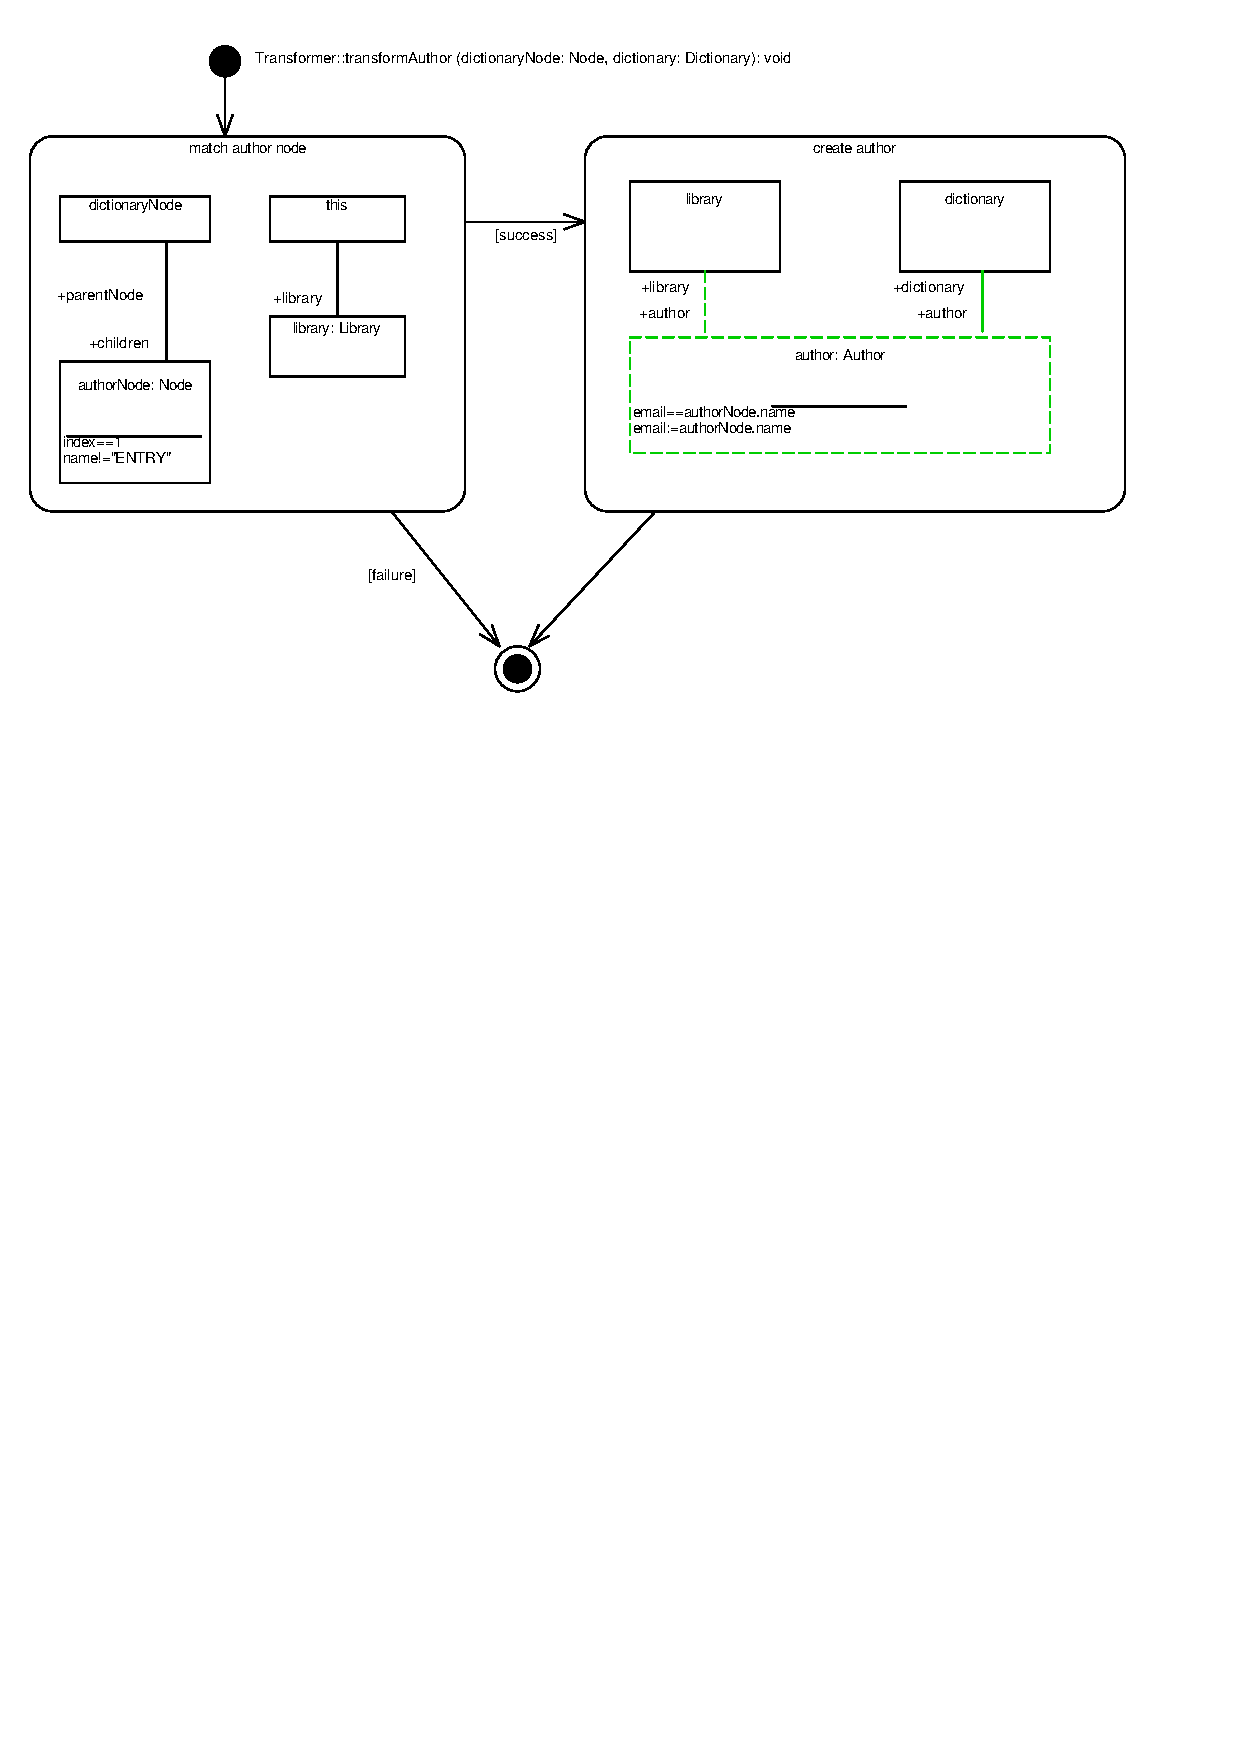
\includegraphics[width=\textwidth]{pics/moca/3MocaTreeToModel/transformAuthorPrint}
  \caption{SDM transformAuthor}
  \label{fig:moca-transformAuthor}
\end{center}
\end{figure}

\clearpage
\item[$\blacktriangleright$] As a final step, open \texttt{MocaMain.java} (Fig.~\ref{fig:moca-8-MocaMain}) and edit lines 32 -- 39 as follows:
\begin{verbatim}
// Transform tree-to-model
Transformer transformer = 
  DictionaryCodeAdapterFactory.eINSTANCE.createTransformer();
Library library = transformer.transformFolder(tree);
  
// Save model to file
eMoflonEMFUtil.saveModel(DictionaryLanguagePackage.eINSTANCE, 
  library, "./instances/library.xmi");  
\end{verbatim}
  
Open and inspect the library model using the reflective model browser and note especially the cross-tree references between authors and their dictionaries. 
\end{enumerate}

%\input{mocaHTML}
 
